\section{Near Neighbor Search}\label{sec:nn}

Fast retrieval of similar patches is crucial for making
construction of a sizeable patch-based database feasible.
This is essentially near-neighbor retrieval in
relatively high dimensions $3 \cdot n^2$ (1875 for $n=25$).
Image retrieval has been addressed in a number of papers,
including more complex feature respresentations ~\cite{perronnin2010large}.
Our poblem is somewhat different from most of previous work
in that the variability
in small patches is much less than in regular-sized images,
and semantic information is irrelevant, and vectors are much shorter
than for regular-sized images.
Thus, we focus on tuning
a simple Locality-Sensitive Hashing variant for our
particular application.

\subsection{Locality-Sensitive Hashing}

Locality-Sensitive Hashing (LSH)~\cite{LSH:Andoni}
is popular approach to approximate near-neighbor search
in high dimensions.
Because this approach is hashing-based, it is
attractive for database applications, where entire lookup data structure
cannot be stored in memory.

At a high-level, LSH applies a family of hash functions $F_i$:

Why we don't want many hash tables:

\begin{equation*}
\begin{aligned}
P[b(P_i) = b(P_j) | S(P_i, P_j < T)] > P_1\\
P[b(P_i) = b(P_j) | S(P_i, P_j) > cT] < P_2
\end{aligned}
\end{equation*}

% Rand proj; right: tables + concat
\begin{figure}[ht!]
\centering
\subfigure[Random projection hashing]{%
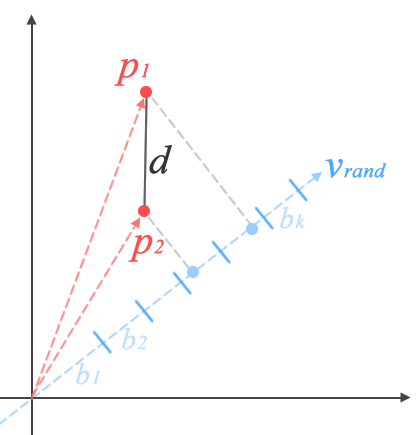
\includegraphics[width=1.5in]{fig_NN/rand_proj.png}
\label{fig:rand-proj}}
\quad
\subfigure[PCA-based hashing]{%
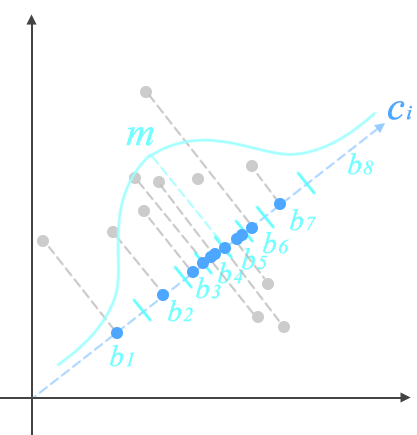
\includegraphics[width=1.5in]{fig_NN/pca_proj.png}
\label{fig:pca-proj}}
\caption{TODO.}
\label{fig:proj}
\end{figure}

\subsection{Near-Neighbor Search with LSH}\label{ssec:nn-lsh}

Using a single amplified hash function $\mathcal{G}$, finding
all likely neighbors of a patch simply amounts to computing
its hash value and taking all the patches that fall into the
same hash bin.
Moreformally, we can define the function
in Alg.~\ref{alg:insert2} as follows:
\begin{algorithmic}[1]
\Statex \texttt{\textbf{FindLikelySimilarPatches}}($P_j$):
\State $h \leftarrow \mathcal{G}$ (\texttt{ToVector($P_j$)})
\State $SimPat \leftarrow$ \texttt{select patch from patch\_dict where id in
(select patch\_id from patch\_hashes where hash = h)}
\end{algorithmic}
Of course, the quality of the result depends heavily on the
properties of the hash function, which is something we discuss next.

\subsection{Naive LSH}\label{sec:naive-nn}

\subsection{PCA-based LSH}

% PCA-based LHS;\\
% 3 distributions\\
% all components

\begin{figure}[ht!]
\centering
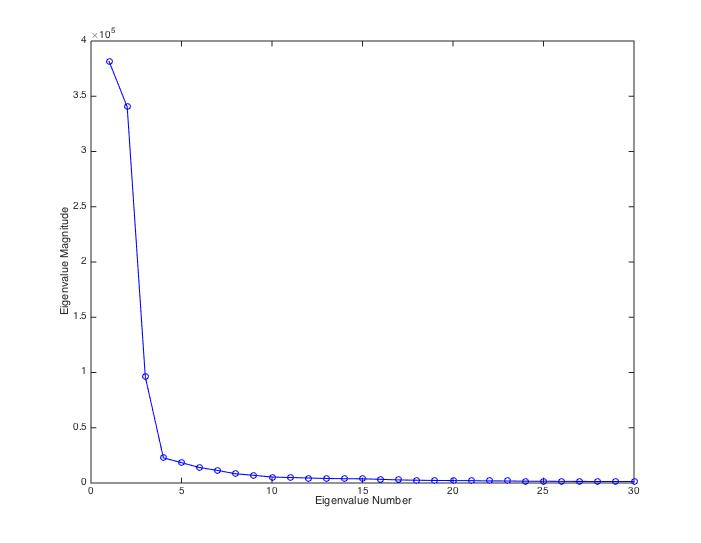
\includegraphics[width=3in]{fig_NN/lambdas.jpg}
\label{fig:lambdas}
\end{figure}

We ran Principal Component Analysis (PCA) on 80K patch vectors
sampled from 1000 images
sampled uinformly from all the categories in the
SUN database~\cite{SUN}.


\subsection{Self-similarity Optimization}

\subsection{Color Uniformity}



\subsection{NN Results and Analysis}

We constructed 3 databases on the same set of
10,000 images sampled
from all categories of the SUN database, with image size
set to 500, and patch size set to 25, using the following
hashing strategies for Near Neighbor(NN) search:\\
\begin{enumerate}
\item \textbf{Naive NN}: 10 random projection vectors sampled from unit Normal with
uniform bin size (outliers truncated)
\item \textbf{PCA NN}: 10 first principla components as projection vectors with
bin size adapted to the distribution of projections
\item \textbf{PCA + U NN}: nearly uniform patches are handled using a separate
hash table, and non-uniform patches handled with PCA NN
\end{enumerate}

To evaluate the results of this, we computed the following metrics.

%FR - found ratio: Count(good match found)/Count(good match not found)

% Table
\begin{table}
\begin{tabular}{ | l | l | l | l | l | l | l | l | }
\hline
& time & \#patches & \#bins & FR & Stime & FPQ & IRQ \\
\hline
Naive NN & & & & & & & \\
PCA NN & 7h27min & 3,309,583 & 2,751,235 & & & &  \\
PCA + U NN & & & & & & &\\
\hline
\end{tabular}
\caption{Results on 10,000 images samples from all
the categories of the SUN database, where the rows
are for naive projection hashing, PCA-based hashing and
PCA-based hashing combine with uniform patch hashing.}
\label{tb:nn-res}
\end{table}

PCA NN: Finished batch-upload of 10000 files in 26827397
NAIVE NN: 7:35AM - 1:50AM for 4367 images
